\documentclass[12pt]{report}

\usepackage{csquotes}
\usepackage[ngerman]{babel}

\usepackage[utf8]{inputenc}
\usepackage{glossaries}
\usepackage{tabto}
\usepackage{verbatimbox}
\usepackage{amsmath}
\usepackage{tabularx}
\usepackage{lscape}
\usepackage{adjustbox}
\usepackage{lipsum}
\usepackage[toc,page]{appendix}
\usepackage{enumitem}
\usepackage{biblatex}

\addbibresource{sample.bib}
\makeglossaries

%\include{chapters/glossary}

\usepackage{geometry}
 \geometry{
 a4paper,
 total={170mm,257mm},
 left=20mm,
 top=20mm,
 }
\usepackage{graphicx}
\usepackage{booktabs}

\usepackage{hyperref}
\hypersetup{
    colorlinks=true,
    linkcolor=black,
    filecolor=black,      
    urlcolor=black,
}


\graphicspath{ {images/} }

\usepackage[pagestyles]{titlesec}
\titleformat{\chapter}[hang]{\normalfont\huge\bfseries}{\thechapter}{1em}{\Huge}
\titlespacing*{\chapter}{0pt}{0pt}{1em}

\titleformat{\section}{\normalfont\Large\bfseries}{\thesection}{1em}{}
\titlespacing*{\section}{0em}{1em}{0em}
\titlespacing*{\chapter}{0pt}{-2\baselineskip}{1em}

\titleformat{\subsection}{\normalfont\large\bfseries}{\thesubsection}{1em}{}
\titleformat{\subsubsection}{\normalfont\normalsize\bfseries}{\thesubsubsection}{1em}{}
\titleformat{\paragraph}[runin]{\normalfont\normalsize\bfseries}{\theparagraph}{1em}{}
\titleformat{\subparagraph}[runin]{\normalfont\normalsize\bfseries}{\thesubparagraph}{1em}{}
\title{
    %\includegraphics[scale=0.8]{content/pictures/BaseLogo.png}\\
    \hfill \break
    {Projektarbeit Artificial Intelligence}\\
    {\large Berner Fachhochschule Departement Technik und Informatik}\\
    {\large Frühlingssemester 2021}\\
    {\large Dozenten: Jürgen Eckerle}\\
}

\author{Manuel Gasser und Julian Haldimann}
\date{\today}

\counterwithout{figure}{chapter}
\counterwithout{table}{chapter}

\begin{document}
    \maketitle

    \chapter{Abstract}
    Die Aufgabe war es dem Agenten einen möglichen Weg zum Schatz zu zeigen. 
Der Schatz ist in einem der verschlossenen Räume versteckt. Der Ort des
Schatzes ist jedoch bekannt. Lediglich der Weg zum Ziel ist ein Rätsel.
Am Ende sollte eine mögliche Route zum Schatz in einer Liste abgebildet
werden. Die Route beinhaltet verschiedene Schlüssel, welche genau in dieser
Reihenfolge augelesen werden müssen um ans Ziel zu kommen. Falls keine Route 
vorhanden ist, wird einfach false zurückgegeben.\\
\\
Damit wir überhaupt mit Prolog unser Projekt umsetzen konnten, mussten wir die 
Modellierung der Räume und der Schlüssel vornehmen. Ohne diese Definition können 
keine Abfragen gemacht werden. Bei der Thematik mit dem Raum und dessen Inhalt,
haben wir uns überlegt für jede Kombination einen separaten Eintrag zu machen. \\
\\
Dasselbe haben wir für verschachelte Räume gemacht. Jeder Raum der einen oder mehrere
Räume enthält hat mindestens eine Definition erhalten. Damit wir von einem Startraum
ausgehen konnten, haben wir einen solchen definiert. Dieser hat in unserem Fall 
die Raumnummer 0. Am Ende der Modellierung haben wir noch definiert, dass sich die 
Schatzkiste im Raum 13 befindet. \\
\\
Am Ende der Arbeit konnten wir eine Weg zum Schatz finden. Der kalkulierte Weg wurde
jedoch noch in einer falschen Reihenfolge ausgegeben und musste noch richtig sortiert
werden. Dazu haben wir einen einfachen Bubblesort verwendet. Sortiert wurde nach Anzahl Schritten,
welche man braucht um an einen Schlüssel zu kommen.

    \tableofcontents
    
    \pagenumbering{arabic}
	\chapter{Einführung}

\section{Projektbeschrieb}
Als Projektarbeit für das Fach Artificial Intelligence haben wir folgende Ausgangssituation
erhalten:\\
\\
\noindent
In einem Labyrinth von verborgenen Räumen befindet sich irgendwo ein Schatz verborgen, 
den es zu finden gilt. Die Türe zu den Räume sich verschlossen und lassen sich nur über 
den passenden Schlüssel öffnen. Räume können verschachtelt sein, das heisst innerhalb 
eines Raumes können weitere Räumen liegen,die ebenfalls durch Türen verschlossen sind.

\begin{figure}[h]
    \begin{center}
        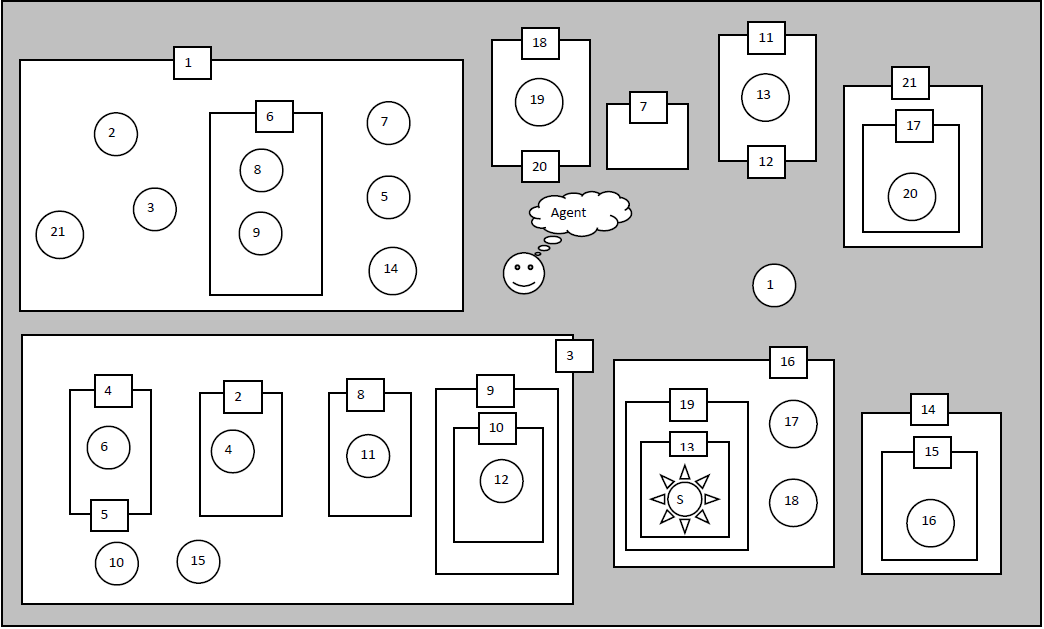
\includegraphics[width=1\textwidth]{content/pictures/situation.png}
        \caption{Ausgangslage}
        \label{fig:situation}
    \end{center}
\end{figure}

\section{Aufgabenstellung}
Folgende Aufgaben gibt es zu lösen in diesem Projekt:
\begin{itemize}
    \item Schreiben Sie ein Prolog-Programm, das unsere obige Problemsituation modellieren unter Annahme, 
    dass die vollständige Information gegeben ist. Es soll möglich sein, mittels Anfragen zu 
    überprüfen, ob eine bestimmte Türe erreichbar ist oder ob ein bestimmter Raum betreten 
    werden kann, usw.
    \item Modellieren Sie unter Verwendung von Listen die Möglichkeit einen Handlungsplan zu erhalten, 
    der aufzeigt, wie die einzelnen Ziele erreicht werden können.
\end{itemize}
\newpage


	\chapter{Ergebnisse}

    \printglossaries

    \listoftables

    \listoffigures
\end{document}
